\section{Subject information}

%-------------------------------------------------------------------------
\subsection*{Subject aims}

The main aim of the subject is to explore the principles, techniques and tools used to analyse, design and implement high integrity systems.
\emph{High integrity systems} are systems that must operate with critical levels of security, safety, reliability, or performance.  The engineering methods required to develop high integrity systems go well beyond the standards for less critical software.

Topics will include:

\begin{itemize}
 \item high integrity system definition;
 \item programming languages for high-integrity systems;
 \item safety and security analysis;
 \item modelling and analysis;
 \item fault tolerance; and
 \item proving program correctness.
\end{itemize}

%-------------------------------------------------------------------------
\subsection*{Subject outcomes}

On completion of this subject students should be able to:

\begin{itemize}

 \item Demonstrate an understanding of the issues facing high    integrity systems developers.

 \item Demonstrate the ability to analyse highly dependable systems and to synthesise    requirements and operating parameters from their analysis.

 \item Demonstrate the ability to choose and make trade-offs between    different software and systems architectures to achieve multiple    objectives.

 \item Develop algorithms and code to meet high integrity    requirements.

  \item Demonstrate the ability to assure high integrity systems.
\end{itemize}


\subsection*{Generic Skills}

The subject is a technical subject. The aim is to explore the various
approaches to building software with specific attributes into a
system.

The subject will also aim to to develop a number of {\em generic
skills}.

\begin{itemize}

  \item We encourage {\em independent research} in order to develop
    your ability to learn independently, assess what you learn, and
    apply what you learn.
  
  \item You will be developing experience at empirical software
    engineering, and the interpretation and assessment of quantitative
    and qualitative data.
  
  \item Finally, and perhaps most importantly, you will be encouraged
    to develop critical analysis skills that will complement and round
    what you have learnt so far in your degree.

\end{itemize}

\subsection*{Preconditions}

The reason for giving preconditions is that the specify the knowledge assumed at the start of the subject and consequently the knowledge and skills upon which the subject builds. Preconditions also allow students from a Universities other than The University of Melbourne and who do not have the formal prerequisites listed above to judge whether or not they have the knowledge required for the subject. 
Specifically the subject assumes:

\begin{enumerate}

 \item Knowledge and experience of software engineering processes and    practices, the risks associated with software and system    development, quality and quality assurance, software process, and    software project management.

  \item Knowledge and experience of requirements elicitation and     analysis techniques, requirements modelling and specification,     use-case modelling, and UML or similar modelling notations.

  \item Knowledge and experience of software architectures,     architectural styles and design patterns, design with UML or     similar graphical notation, developing code to meet architectural     and detailed designs.

  \item Knowledge and experience of discrete mathematics, including     predicate logic and formal proof.

\end{enumerate}


%-------------------------------------------------------------------------
\subsection*{Subject staff}

Tim Miller\\
Email: {\tt tmiller@unimelb.edu.au}\\
Office: DMD 6.09\\
You can drop by my office any time to see if I am in. If you do not want to chance it, email me for an appointment.

Vanessa Teague\\
Office: DMD 9.18\\ 
Email: \texttt{vjteague@unimelb.edu.au}

 Qingyu Chenn\\
 Email: \texttt{qingyuc1@student.unimelb.edu.au}

\subsection*{Resources}

LMS: all assignment sheets, notes, tutorial/workshop sheets, and announcements will be put on the LMS: \url{http://www.lms.unimelb.edu.au/}.


\subsection*{Contact hours}

\begin{itemize}

 \item Lectures: 2 hours, one one Tuesday and one on Wednesday

 \item Tutorial/workshop: 1 hour on Tuesday. These start in week 2.

\end{itemize}

It is expected that you will attend lectures and tutorials regularly. Lectures
will be made available via Lectopia, but given the lecturer style of the
subject coordinator, these may not be so useful.


%-------------------------------------------------------------------------
\subsection*{Assessment}

Four assignments, totalling 50\%:

\begin{itemize}

 \item Assignment 1: Designing and implementing a high integrity system in Ada.

 \item Assignment 2: Performing a safety analysis on a system, and arguing that certain properties hold (done in pairs).

 \item Assignment 3: Constructing a security model and a fault-tolerant design of a high integrity system.

 \item Assignment 4: Proving correctness and measuring the reliability of a fault tolerant system.

\end{itemize}

A two-hour end-of-semester examination, worth 50\%.

\emph{You must receive 25/50 for assignments and 25/50 on the exam to pass the subject.}

%-------------------------------------------------------------------------
\section{Introduction to high integrity systems}

\subsection*{What is a high integrity system?}

High integrity systems a software controlled systems in which, in the event they fail, could result in harm to humans (including loss of life), harm on the environment, mass destruction of property, or harm to society in general.

There are four broad areas that are commonly considered as high integrity systems:

\begin{itemize}

 \item \emph{Safety-critical systems:} Systems whose failure may result in harm to humans or the environment.  Examples include aerospace systems, medical devices, automotive systems, power systems, and railway systems.

 \item \emph{Security-critical systems}: Systems whose failure may result in breach of security. Examples include defence systems, government data stores.

 \item \emph{Mission-critical systems}: Systems whose failure may result in the failure of some deliberative missions. Examples include navigation systems on autonomous aerospace vehicles, computer-aided dispatch systems (e.g. in emergency services), and  command-and-control systems in armed forces.

  \item \emph{Business-critical systems:} Systems whose failure may result in extreme financial loss to a business or businesses. Examples include stock exchange systems, trade platforms, and even accounting systems (e.g. in a bank).

\end{itemize}


%-------------------------------------------------------------------------
\subsection*{What is high integrity systems engineering?}

The high impact of failure of a high integrity system means that the software controlling the system must be highly \emph{dependable}. The standard software engineering methods used for constructing good software systems typically do not lead to such dependability. As such, specialised methods for engineering software are required for high integrity systems.


Avizienis et al.'s work on dependability attributes help us to
understand high integrity systems based on six key attributes, shown in Figure~\ref{fig:intro:dependenability}. For a single high integrity system, one or more of the above attributes will be of high importance.

\begin{figure}
\centering
  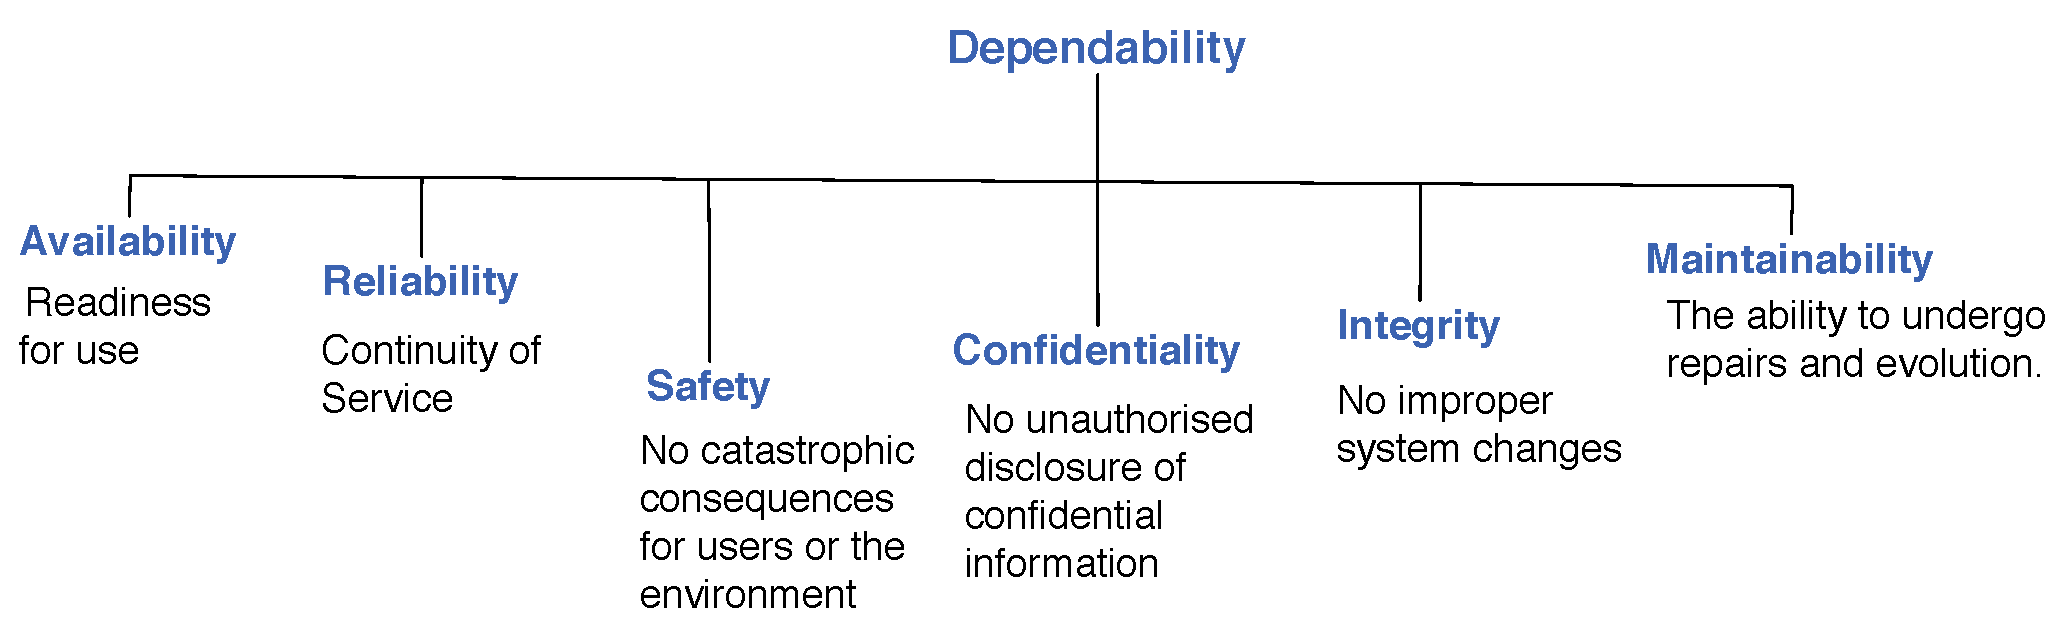
\includegraphics[scale=0.45]{\rootdir/intro/figures/dependability}
 \caption{Dependability model from ``\emph{Avizienis, Laprie \& Randell: Fundamental
    Concepts of Reliability''}}
 \label{fig:intro:dependenability}
\end{figure}



%-------------------------------------------------------------------------
\subsection*{How do we achieve high-integrity?}

High integrity is achieved using a combination of:

\begin{itemize}

 \item {\em Rigorous engineering processes}, such as strict configuration management, auditing, and review process. We will not introduce any new theory on these topics in this subject.

 \item {\em Specialised analysis and design methods}, such as safety \& hazard analysis and fault prediction methods. These will be covered in Part II of the subject.

 \item {\em Specialised modelling and analysis methods/notations}, such as mathematical logic and set theory. These will be covered in Part III of the subject.

 \item {\em Fault tolerant design methods}, such as redundancy, design diversity, and fault detection mechanisms. These will be covered in Part IV of the subject.

 \item \emph{Specialised assurance methods}, such as model checking, proof, and model-based testing. These will be covered in Part V of the subject.

\end{itemize}

%-------------------------------------------------------------------------
\subsection*{How do we achieve high-integrity?}

Methods that are otherwise considered too expensive to apply to ``standard'' software systems become cost-effective in high integrity domains. This is because the cost of failure far outweighs the effort involved required to engineer a dependable product.

Of importance is that high dependability cannot be demonstrated by just running large set of tests. Although testing still plays an important role in high integrity systems, a really large set of tests is still usually only a fraction of all possible behaviour. As such, testing does not demonstrate dependability.

Perhaps the important lesson to learn from this introduction is:

\begin{quote}
``\emph{Program testing can be used to show the presence of bugs, but never to show their absence!}'' --- Edsger W. Dijkstra \cite{dijkstra1970notes}.
\end{quote}


\section{Subject outline}

Now that we have a better idea about high integrity systems engineering, we define the subject outline:

\begin{enumerate}[\bf {Part} I:]

 \item Introduction to high integrity systems.

 \item Safety- and security-critical systems.

   Topics will be drawn from: safety engineering, and accident \& hazard analysis for high-integrity systems; security analysis, cryptography.

 \item  Modelling and analysis.

  Topics will be drawn from: discrete maths for software engineering, model-based specification and analysis, proof, and lightweight verification.

 \item High integrity systems design.

  Topics will be drawn from: reliability, fault detection, fault containment, fault tolerant design, and design by contract.

 \item Assurance.

  Topics will be drawn from: proving program correctness, programming languages for high integrity systems, safe-subset programming languages, programming tools for high integrity verification, and   model-based testing.

\end{enumerate}

% LocalWords:  elicitation UML DMD LMS Lectopia Avizienis al Laprie maths
% LocalWords:  practices et Edsger
